\chapter{Ubundet Optimalisering}\label{chap:unconstrained_optimization}

Ubundet optimalisering (eller fri optimalisering) refererer til problemer uten eksplisitte restriksjoner på variablene.
Målet er å minimere en \textit{glatt objektfunksjon} \( f : \mathbb{R}^n \to \mathbb{R} \) over hele \(\mathbb{R}^n\):

\[
  \min_{\symbf{x} \in \mathbb{R}^n} f(\symbf{x}),
\]

hvor løsningen \(\symbf{x}^*\) tilfredsstiller

\[
  f(\symbf{x}^*) \;\le\; f(\symbf{x})
  \quad \forall \symbf{x} \in \mathbb{R}^n.
\]

\paragraph{Egenskaper ved ubundet optimalisering}

\begin{itemize}
  \item \textbf{Ingen restriksjoner}: Den tillatte mengden (feasible set) er hele \(\mathbb{R}^n\), uten likhets- eller ulikhetsbetingelser.
  \item \textbf{Enklere oppsett}: Det er ikke behov for å håndtere restriksjoner i selve problemet.
  \item \textbf{Fokuserer kun på målfunksjonen}: Algoritmer søker etter punkter \(\symbf{x}\) som reduserer \(f(\symbf{x})\) direkte, uten å ta hensyn til andre forhold.
\end{itemize}

\section{Stasjonære punkter}\label{sec:stationary_points}

\begin{definition}{Stasjonære punkter}{stationary_points}
  Et punkt \(\symbf{x}^*\) er et stasjonært punkt for \(f\) dersom gradienten \(\nabla f(\symbf{x}^*) = 0\).
\end{definition}

\subsection*{Konvergens til stasjonære punkter}
For å sikre konvergens til en stasjonær løsning \(\symbf{x}^*\), må følgende betingelser typisk oppfylles:
\begin{enumerate}
  \item \(f(\symbf{x})\) er kontinuerlig deriverbar (\(C^1\)).
  \item Gradienten \(\nabla f(\symbf{x})\) eksisterer og er Lipschitz-kontinuerlig.
  \item \hyperref[def:level_set]{Nivåsettene} \(\mathcal{L}_f(\alpha)\) er begrenset og lukkede \hyperref[def:compact_set]{(kompakte)}.
\end{enumerate}

Under disse antagelsene sikres konvergens til en stasjonær løsning \(\symbf{x}^*\) der
\(\nabla f(\symbf{x}^*) = 0\).
Dette innebærer at
\[
  \lim_{k \to \infty} \|\nabla f(\symbf{x}_k)\| = 0,
\]
hvor \(\symbf{x}_k\) er iteratene generert av en optimaliseringsalgoritme, og \(\symbf{x}^*\) tilfredsstiller de førsteordens nødvendige betingelsene \(\nabla f(\symbf{x}^*) = 0\).

\section{Trust Region Metoder}

Trust region-metoder er en annen tilnærming til optimalisering. Istedenfor å velge en retning og deretter en steplengde, definerer vi en region hvor vi "stoler på" en approksimasjon av funksjonen.

\begin{definition}{Trust Region}{trust_region}
  Trust region-metoder løser et begrenset optimaliseringsproblem:
  \[
    \min_{p \in \mathbb{R}^n} m_k(p) \quad \text{slik at} \quad \|p\| \leq \Delta_k
  \]
  hvor $m_k$ er en modell (typisk kvadratisk) av $f$ nær $x_k$ og $\Delta_k > 0$ er trust region-radius.
\end{definition}

\subsection{Trust Region Algoritme}

\begin{enumerate}
  \item Velg initial $x_0$ og $\Delta_0 > 0$, sett $k = 0$
  \item Lag en modell $m_k(p)$ nær $x_k$, typisk:
        \[
          m_k(p) = f(x_k) + \nabla f(x_k)^T p + \frac{1}{2}p^T B_k p
        \]
  \item Løs (approksimativt) trust region-delproblemet:
        \[
          p_k = \arg\min_{p \in \mathbb{R}^n} m_k(p) \quad \text{slik at} \quad \|p\| \leq \Delta_k
        \]
  \item Beregn ratioen av faktisk til predikert reduksjon:
        \[
          \rho_k = \frac{f(x_k) - f(x_k + p_k)}{m_k(0) - m_k(p_k)}
        \]
  \item Oppdater $x_k$ og $\Delta_k$ basert på $\rho_k$:
        \begin{itemize}
          \item Hvis $\rho_k$ er stor: aksepter steget og øk $\Delta_k$
          \item Hvis $\rho_k$ er moderat: aksepter steget men behold $\Delta_k$
          \item Hvis $\rho_k$ er liten: avvis steget og reduser $\Delta_k$
        \end{itemize}
\end{enumerate}

\begin{figure}[H]
  \centering
  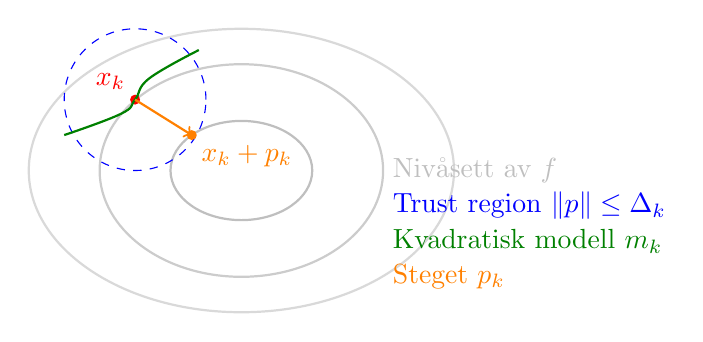
\begin{tikzpicture}[scale=0.9]
    % Contours of the function
    \draw[gray!30, thick] (0,0) ellipse (3 and 2);
    \draw[gray!40, thick] (0,0) ellipse (2 and 1.5);
    \draw[gray!50, thick] (0,0) ellipse (1 and 0.7);

    % Current point
    \fill[red] (-1.5,1) circle (2pt) node[above left]{$x_k$};

    % Trust region
    \draw[blue, dashed] (-1.5,1) circle (1);

    % Model approximation
    \draw[green!50!black, thick] plot[smooth, tension=0.7] coordinates {(-2.5,0.5) (-1.7,0.8) (-1.5,1) (-1.3,1.3) (-0.6,1.7)};

    % Optimal step within trust region
    \draw[->, thick, orange] (-1.5,1) -- (-0.7,0.5);
    \fill[orange] (-0.7,0.5) circle (2pt) node[below right]{$x_k + p_k$};

    % Legend
    \node[gray!50, right] at (2,0) {Nivåsett av $f$};
    \node[blue, right] at (2,-0.5) {Trust region $\|p\| \leq \Delta_k$};
    \node[green!50!black, right] at (2,-1) {Kvadratisk modell $m_k$};
    \node[orange, right] at (2,-1.5) {Steget $p_k$};
  \end{tikzpicture}
  \caption{Trust region-metoden.
    Det blå sirkelen viser det tillatte området (Trust region) rundt $x_k$,
    og det oransje steget er løsningen av delproblemet.}
\end{figure}

\subsection{Trust Region vs. Linjesøk}
\begin{itemize}
  \item \textbf{Trust Region}: Først bestemmes hvor langt vi kan gå (radius $\Delta_k$), deretter bestemmes retningen og steplengden samtidig.
  \item \textbf{Linjesøk}: Først bestemmes retningen $p_k$, deretter bestemmes hvor langt vi skal gå i den retningen (steplengde $\alpha_k$).
\end{itemize}

Trust region-metoder er spesielt robuste når Hessian-matrisen ikke er positiv definit, da de naturlig håndterer negative krumninger ved å begrense steglengden.

\section{Linjesøk}\label{sec:line_search}

Linjesøk er en metode for å finne minimum av en funksjon \(f\) ved å iterere over retninger og steplengder.

Ideen er å velge en retning \(p_k\) og deretter finne en passende steplengde \(\alpha_k\) langs denne retningen.

\begin{definition}{Linjesøk}{line_search}
  Gitt en nåværende iterasjon \(x_k\) og en søkeretning \(p_k\), finner linjesøk en steglengde \(\alpha_k > 0\) slik at
  \[
    x_{k+1} = x_k + \alpha_k p_k
  \]
  gir tilstrekkelig reduksjon i målfunksjonen \(f\).
\end{definition}

For å oppnå dette, må vi oppfylle visse betingelser for \(\alpha_k\).
De varierer i hvor strenge krav de stiller til reduksjonen i funksjonsverdien, gradientens/Hesse-matrisens oppførsel og forholdet mellom disse.
De mest kjente er Wolfe-betingelsene, Armijo-betingelsen, Goldstein-betingelsen, kurvbetingelsen og Strong Wolfe-betingelsene.

\subsection{Wolfe-betingelser}

For å sikre tilstrekkelig forbedring, brukes ofte Wolfe betingelsene:

\begin{align}
  f(x_k + \alpha_k p_k)              & \leq f(x_k) + c_1 \alpha_k \nabla f(x_k)^T p_k \tag{Armijo betingelse} \\
  \nabla f(x_k + \alpha_k p_k)^T p_k & \geq c_2 \nabla f(x_k)^T p_k \tag{Krumningsbetingelse}
\end{align}

der \(0 < c_1 < c_2 < 1\) er konstanter, typisk \(c_1 \approx 10^{-4}\) og \(c_2 \approx 0.9\).

\begin{definition}{Wolfe-betingelsene}{wolfe_conditions}
  \begin{enumerate}
    \item \textbf{Armijo-betingelsen}:
          \[
            f(\symbf{x} + \alpha \symbf{d})
            \;\le\;
            f(\symbf{x})
            \;+\;
            \beta\,\alpha\,\nabla f(\symbf{x})^T \symbf{d}.
          \]
    \item \textbf{Krav til avtagende rate}:
          \[
            \nabla f(\symbf{x} + \alpha \symbf{d})^T \symbf{d}
            \;\ge\;
            \rho \,\nabla f(\symbf{x})^T \symbf{d}.
          \]
  \end{enumerate}
\end{definition}

\subsection{Armijo-betingelsen}
\begin{definition}{Armijo-betingelsen}{armijo_condition}
  Armijo-betingelsen sikrer at steget gir en tilstrekkelig reduksjon i funksjonsverdien. Den krever at
  \[
    f(\symbf{x} + \alpha \symbf{d})
    \;\le\;
    f(\symbf{x})
    \;+\;
    \beta\,\alpha\,\nabla f(\symbf{x})^T \symbf{d},
  \]
  hvor \(\beta\) er en liten positiv konstant. Dette tilsier at \(f\) reduseres i tråd med en lineær modell.
\end{definition}

\begin{figure}[h]
  \centering
  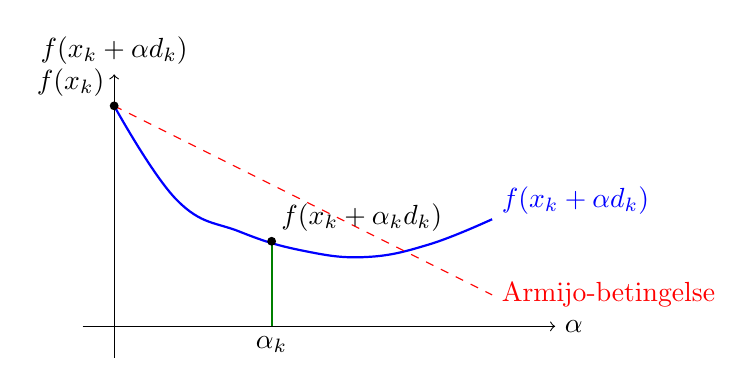
\begin{tikzpicture}[scale=0.8]
    % Axis
    \draw[->] (-0.5,0) -- (7,0) node[right]{$\alpha$};
    \draw[->] (0,-0.5) -- (0,4) node[above]{$f(\symbf{x}_k + \alpha \symbf{d}_k)$};

    % Function curve
    \draw[thick, blue] plot[smooth, tension=0.7] coordinates {(0,3.5) (1,2) (2,1.5) (3,1.2) (4,1.1) (5,1.3) (6,1.7)};

    % Armijo condition line
    \draw[red, dashed] plot coordinates {(0,3.5) (6,0.5)};

    % Initial point
    \fill (0,3.5) circle (2pt) node[above left]{$f(\symbf{x}_k)$};

    % Step point
    \draw[green!50!black, thick] (2.5,0) -- (2.5,1.35);
    \fill (2.5,1.35) circle (2pt) node[above right]{$f(\symbf{x}_k + \alpha_k \symbf{d}_k)$};

    % Step length label
    \node[below] at (2.5,0) {$\alpha_k$};

    % Legend
    \node[blue, right] at (6,2) {$f(\symbf{x}_k + \alpha \symbf{d}_k)$};
    \node[red, right] at (6,0.5) {Armijo-betingelse};
  \end{tikzpicture}
  \caption{Illustrasjon av linjesøk. Den blå kurven viser funksjonen langs søkeretningen, mens den røde stiplede linjen viser Armijo-betingelsen. Steglengden $\alpha_k$ gir tilstrekkelig reduksjon.}
\end{figure}

\subsection{Goldstein-betingelsen}
\begin{definition}{Goldstein-betingelsen}{goldstein_condition}
  Goldstein-betingelsen krever at den nye funksjonsverdien etter steget ligger innenfor et avgrenset intervall:
  \[
    f(\symbf{x}) + (1-\beta)\,\alpha\,\nabla f(\symbf{x})^T \symbf{d}
    \;\le\;
    f(\symbf{x} + \alpha \symbf{d})
    \;\le\;
    f(\symbf{x}) + \beta\,\alpha\,\nabla f(\symbf{x})^T \symbf{d}.
  \]
  Dette forhindrer at vi tar et for lite eller for stort steg.
\end{definition}

\subsection{Kurvbetingelsen}
\begin{definition}{Curvature-betingelsen}{curvature_condition}
  Kurvbetingelsen ser på gradientens endring etter steget og krever
  \[
    \bigl|\nabla f(\symbf{x} + \alpha \symbf{d})^T \symbf{d}\bigr|
    \;\le\;
    -\sigma \,\nabla f(\symbf{x})^T \symbf{d},
  \]
  for en konstant \(\sigma \in (0,1)\). Dette sikrer at gradienten ikke endrer retning for brått, og at man unngår “overkorrigering”.
\end{definition}

\subsection{Strong Wolfe-betingelsene}
\begin{definition}{Strong Wolfe-betingelsene}{strong_wolfe_conditions}
  Strong Wolfe-betingelsene kombinerer Armijo-betingelsen med en kurvbetingelse:
  \begin{enumerate}
    \item Armijo-betingelsen:
          \[
            f(\symbf{x} + \alpha \symbf{d})
            \;\le\;
            f(\symbf{x})
            \;+\;
            \beta\,\alpha\,\nabla f(\symbf{x})^T \symbf{d}.
          \]
    \item Kurvbetingelsen:
          \[
            \bigl|\nabla f(\symbf{x} + \alpha \symbf{d})^T \symbf{d}\bigr|
            \;\le\;
            -\sigma \,\nabla f(\symbf{x})^T \symbf{d}.
          \]
  \end{enumerate}
\end{definition}

\subsection{Goldstein-Wolfe-betingelsene}
\begin{definition}{Goldstein-Wolfe-betingelsene}{goldstein_wolfe_conditions}
  Goldstein-Wolfe-betingelsene krever at Armijo- og Goldstein-betingelsene begge er oppfylt:
  \begin{enumerate}
    \item Armijo-betingelsen:
          \[
            f(\symbf{x} + \alpha \symbf{d})
            \;\le\;
            f(\symbf{x})
            \;+\;
            \beta\,\alpha\,\nabla f(\symbf{x})^T \symbf{d}.
          \]
    \item Goldstein-betingelsen:
          \[
            f(\symbf{x}) + (1-\beta)\,\alpha\,\nabla f(\symbf{x})^T \symbf{d}
            \;\le\;
            f(\symbf{x} + \alpha \symbf{d})
            \;\le\;
            f(\symbf{x}) + \beta\,\alpha\,\nabla f(\symbf{x})^T \symbf{d}.
          \]
  \end{enumerate}
\end{definition}

\subsection{Eksakt vs Ikke-Eksakt Linjesøk}

\begin{itemize}
  \item \textbf{Eksakt linjesøk}: Finn $\alpha_k$ som minimerer $f(x_k + \alpha p_k)$. Dette er ofte beregningsmessig dyrt.
  \item \textbf{Ikke-eksakt linjesøk}: Finn $\alpha_k$ som gir tilstrekkelig reduksjon, f.eks. ved å oppfylle Wolfe betingelsene.
\end{itemize}

Linjesøk omfatter metoder for å finne en egnet skrittlengde \(\alpha\) eller \(\alpha_k\) i en gitt retning \(\symbf{d}\) som reduserer objektfunksjonen \(f(\symbf{x})\).

\subsection{Backtracking Line Search (BLS)}
Backtracking Line Search er en metode for å finne en passende skrittlengde \(\alpha\) som sikrer en ønsket reduksjon i \(f(\symbf{x})\) langs en retning \(\symbf{d}\).

\subsubsection{Algoritme}
\begin{algorithm}[H]
  \SetAlgoLined
  \KwIn{Startpunkt \( \symbf{x} \), retning \( \symbf{d} \), initial skrittlengde \( \alpha \), \textit{backtracking}-parameter \( \beta \in (0,1) \), \textit{skalering} \( \rho \in (0,1) \)}
  \KwOut{Skrittlengde \( \alpha \)}
  \While{\( f(\symbf{x} + \alpha \symbf{d}) > f(\symbf{x}) + \beta \,\alpha \,\nabla f(\symbf{x})^T \symbf{d} \)}{
    \(\alpha \leftarrow \rho \,\alpha\)
  }
  \caption{Backtracking Line Search (BLS)}
  \label{alg:backtracking_line_search}
\end{algorithm}

\subsection{Konvergens av Linjesøk}
\begin{theorem}{Konvergens av linjesøk}{line_search_convergence}
  Anta at \(f\) er kontinuerlig deriverbar og at det finnes en \(\alpha^* > 0\) slik at
  \[
    f(\symbf{x} + \alpha^* \symbf{d}) < f(\symbf{x}) + \beta\,\alpha^*\,\nabla f(\symbf{x})^T \symbf{d}.
  \]
  Da vil Backtracking Line Search konvergere til en skrittlengde \(\alpha_k\) som tilfredsstiller Armijo-betingelsen.
\end{theorem}

\section{Newtons Metode}\label{sec:newtons_method}

Newtons metode er en iterativ tilnærming for å finne lokale ekstremalpunkter i en funksjon. Den bruker andreordens informasjon (Hesse-matrisen) for å avlede en søkeretning som ofte gir raskere konvergens enn gradientbaserte metoder alene.

\subsection{Algoritme}
Gitt en startverdi \( \symbf{x}_0 \), genererer Newtons metode en sekvens av iterasjoner:
\[
  \symbf{x}_{k+1}
  \;=\;
  \symbf{x}_k
  \;-\;
  [\nabla^2 f(\symbf{x}_k)]^{-1} \,\nabla f(\symbf{x}_k),
\]
der:
\begin{itemize}
  \item \(\symbf{x}_{k+1}\) er neste iterasjon.
  \item \(\nabla f(\symbf{x}_k)\) er gradienten av \(f\) evaluert i \(\symbf{x}_k\).
  \item \(\nabla^2 f(\symbf{x}_k)\) er Hesse-matrisen av \(f\) i \(\symbf{x}_k\).
\end{itemize}

\paragraph{Søkeretning}
Søkeretningen finnes ved:
\[
  \symbf{d}_k
  \;=\;
  -[\nabla^2 f(\symbf{x}_k)]^{-1}\,\nabla f(\symbf{x}_k).
\]
\paragraph{Oppdatering}
\[
  \symbf{x}_{k+1}
  \;=\;
  \symbf{x}_k + \alpha_k \,\symbf{d}_k,
\]
\subparagraph{Skrittlengde}
Skrittlengden \(\alpha_k\) kan finnes ved linjesøk (f.eks.\ Backtracking Line Search).

\begin{algorithm}[H]
  \SetAlgoLined
  \KwIn{Startpunkt \( \symbf{x}_0 \), toleranse \( \epsilon \), maks antall iterasjoner \( K \)}
  \KwOut{Omtrentelig løsning \( \symbf{x}^* \)}
  \For{\( k = 0, 1, 2, \ldots, K\)}{
  Beregn søkeretning:
  \(\symbf{d}_k
  = -[\nabla^2 f(\symbf{x}_k)]^{-1}\,\nabla f(\symbf{x}_k)\)\;
  Finn skrittlengde \(\alpha_k\) (f.eks.\ ved Backtracking Line Search)\;
  Oppdater \(
  \symbf{x}_{k+1}
  = \symbf{x}_k + \alpha_k \symbf{d}_k
  \)\;
  \If{\(\|\nabla f(\symbf{x}_{k+1})\| < \epsilon\)}{
    \Return \(\symbf{x}_{k+1}\)\;
  }
  }
  \caption{Newtons metode}
\end{algorithm}

\subsection{Konvergens av Newtons Metode}
Newtons metode kan konvergere lokalt kvadratisk under visse forutsetninger. La \( f : \mathbb{R}^n \to \mathbb{R} \) være to ganger kontinuerlig deriverbar. Anta at:

\begin{enumerate}
  \item Det finnes et \(\symbf{x}^*\) slik at \(\nabla f(\symbf{x}^*) = 0\).
  \item Hesse-matrisen \(\nabla^2 f(\symbf{x}^*)\) er regulær (invertibel).
  \item \(\nabla^2 f\) er Lipschitz-kontinuerlig i et nabolag rundt \(\symbf{x}^*\); dvs.\ det finnes \( L > 0 \) slik at
        \[
          \| \nabla^2 f(\symbf{x}) - \nabla^2 f(\symbf{y}) \|
          \;\le\;
          L\,\|\symbf{x} - \symbf{y}\|,
        \]
        for alle \(\symbf{x}, \symbf{y}\) i dette nabolaget.
\end{enumerate}

Da kan man vise at for en startverdi \(\symbf{x}_0\) nær \(\symbf{x}^*\), vil Newtons metode konvergere kvadratisk mot \(\symbf{x}^*\).

\begin{proof}{}{}
  La \(\symbf{e}_k = \symbf{x}_k - \symbf{x}^*\) være feilen ved iterasjon \(k\).
  Ved Taylor-utvidelse av gradienten får vi:
  \[
    \nabla f(\symbf{x}_k)
    = \nabla^2 f(\symbf{x}^*)\,(\symbf{x}_k - \symbf{x}^*) + r(\symbf{x}_k),
  \]
  hvor \(\|r(\symbf{x}_k)\|\) er \(\mathcal{O}(\|\symbf{e}_k\|^2)\). Newtons oppdateringsregel er
  \[
    \symbf{x}_{k+1}
    = \symbf{x}_k
    - [\nabla^2 f(\symbf{x}_k)]^{-1}\,\nabla f(\symbf{x}_k).
  \]
  I et lite nabolag av \(\symbf{x}^*\) kan vi anta at
  \(\nabla^2 f(\symbf{x}_k)\approx \nabla^2 f(\symbf{x}^*)\), slik at
  \[
    \symbf{e}_{k+1}
    \;=\; \symbf{x}_{k+1} - \symbf{x}^*
    \;\approx\;
    -[\nabla^2 f(\symbf{x}^*)]^{-1}\,r(\symbf{x}_k).
  \]
  Dermed blir
  \[
    \|\symbf{e}_{k+1}\|
    \;\lesssim\;
    \|[\nabla^2 f(\symbf{x}^*)]^{-1}\|\,
    \|r(\symbf{x}_k)\|
    \;\le\;
    C \|\symbf{e}_k\|^2,
  \]
  for en konstant \(C>0\). Dette illustrerer \textit{kvadratisk konvergens} når \(\symbf{x}_0\) er nært \(\symbf{x}^*\).
\end{proof}

\subsection{Bevis for Kvadratisk Konvergens}
\label{sec:newton_quadratic_convergence}
Argumentet ovenfor kan formuleres mer detaljert ved å vise at feilen \(\|\symbf{e}_{k+1}\|\) er proporsjonal med \(\|\symbf{e}_k\|^2\). Dette er selve definisjonen av kvadratisk konvergens.

\subsection{Kommentarer}
Beviset forutsetter at startverdien \(\symbf{x}_0\) er tilstrekkelig nær \(\symbf{x}^*\). I praksis benyttes ofte modifikasjoner, som for eksempel \textit{dempet Newton} (med linjesøk), for å sikre global konvergens før man oppnår den raske, lokale konvergensfasen.

\subsection{Egenskaper}
\begin{itemize}
  \item \textbf{Kvadratisk konvergens}: Under gitte forutsetninger dobles antall riktige sifre omtrent for hver iterasjon.
  \item \textbf{Krever andreordens deriverbarhet}: \(\nabla^2 f(\symbf{x})\) må eksistere og være invertibel.
  \item \textbf{Beregning kan være kostbar}: Å beregne og invertere \(\nabla^2 f(\symbf{x})\) er dyrt, spesielt i store dimensjoner.
  \item \textbf{Global vs.\ lokal konvergens}: Metoden garanterer ikke nødvendigvis global konvergens uten videre tiltak.
\end{itemize}

\subsection{Modifikasjoner}
\begin{itemize}
  \item \textbf{Dempet Newtons metode}: Benytter en skrittlengde \(\alpha_k\) (linjesøk) for å unngå for store steg.
  \item \textbf{Kvasi-Newton-metoder}: Reduserer kostnader ved å approksimere Hesse-matrisen (f.eks.\ BFGS, DFP).
\end{itemize}


\section{Konjugerte Gradientmetode (CG)}\label{sec:conjugate_gradient}

Konjugert Gradient (CG) metoden er en effektiv iterativ algoritme for å løse lineære ligningssystemer og optimere kvadratiske funksjoner. Den er spesielt nyttig for store, men sparse systemer.

\subsection{Grunnleggende Konsept}
CG-metoden genererer en sekvens av retninger som er konjugerte med hensyn til en symmetrisk, positiv definit matrise. For en kvadratisk funksjon:
\[
  f(\symbf{x}) = \frac{1}{2}\symbf{x}^T\symbf{A}\symbf{x} - \symbf{b}^T\symbf{x} + c,
\]
hvor \(\symbf{A}\) er symmetrisk, positiv definit, søker CG-metoden å løse \(\nabla f(\symbf{x}) = \symbf{A}\symbf{x} - \symbf{b} = \symbf{0}\).

\subsection{CG-algoritme}

\begin{algorithm}[H]
  \SetAlgoLined
  \KwIn{Startpunkt \(\symbf{x}_0\), toleranse \(\epsilon > 0\)}
  \KwOut{Omtrentelig løsning \(\symbf{x}^*\)}
  \(\symbf{r}_0 \gets \symbf{b} - \symbf{A}\symbf{x}_0\) \tcc*{Residual}
  \(\symbf{p}_0 \gets \symbf{r}_0\) \tcc*{Første søkeretning}
  \For{\(k = 0, 1, 2, \ldots\)}{
    \If{\(\|\symbf{r}_k\| < \epsilon\)}{
      \Return \(\symbf{x}_k\) \tcc*{Konvergens oppnådd}
    }
    \(\alpha_k \gets \frac{\symbf{r}_k^T\symbf{r}_k}{\symbf{p}_k^T\symbf{A}\symbf{p}_k}\) \tcc*{Optimal skrittlengde}
    \(\symbf{x}_{k+1} \gets \symbf{x}_k + \alpha_k\symbf{p}_k\) \tcc*{Oppdater løsning}
    \(\symbf{r}_{k+1} \gets \symbf{r}_k - \alpha_k\symbf{A}\symbf{p}_k\) \tcc*{Oppdater residual}
    \(\beta_{k+1} \gets \frac{\symbf{r}_{k+1}^T\symbf{r}_{k+1}}{\symbf{r}_k^T\symbf{r}_k}\) \tcc*{Konjugasjonsparameter}
    \(\symbf{p}_{k+1} \gets \symbf{r}_{k+1} + \beta_{k+1}\symbf{p}_k\) \tcc*{Ny søkeretning}
  }
  \caption{Konjugert Gradient Metode (CG)}
\end{algorithm}

\subsection{Ikke-lineær Konjugert Gradient Metode (Non-Linear CG)}

For generelle ikke-lineære funksjoner tilpasses algoritmen:

\begin{algorithm}[H]
  \SetAlgoLined
  \KwIn{Startpunkt \(\symbf{x}_0\), toleranse \(\epsilon > 0\)}
  \KwOut{Omtrentelig løsning \(\symbf{x}^*\)}
  \(\symbf{g}_0 \gets \nabla f(\symbf{x}_0)\) \tcc*{Gradient}
  \(\symbf{p}_0 \gets -\symbf{g}_0\) \tcc*{Første søkeretning}
  \For{\(k = 0, 1, 2, \ldots\)}{
    \If{\(\|\symbf{g}_k\| < \epsilon\)}{
      \Return \(\symbf{x}_k\) \tcc*{Konvergens oppnådd}
    }
    Finn \(\alpha_k\) ved linjesøk som minimerer \(f(\symbf{x}_k + \alpha\symbf{p}_k)\) \;
    \(\symbf{x}_{k+1} \gets \symbf{x}_k + \alpha_k\symbf{p}_k\) \tcc*{Oppdater løsning}
    \(\symbf{g}_{k+1} \gets \nabla f(\symbf{x}_{k+1})\) \tcc*{Ny gradient}
    Beregn \(\beta_{k+1}\) \tcc*{f.eks. FR eller PR}\;
    \(\symbf{p}_{k+1} \gets -\symbf{g}_{k+1} + \beta_{k+1}\symbf{p}_k\) \tcc*{Ny søkeretning}
  }
  \caption{Ikke-lineær Konjugert Gradient Metode (Non-Linear CG)}
\end{algorithm}

\subsection{Valg av beta-parameter}

Flere formler eksisterer for \(\beta\) i ikke-lineære CG-metoder:
\begin{itemize}
  \item \textbf{Fletcher-Reeves}: \(\beta_{k+1}^{FR} = \frac{\symbf{g}_{k+1}^T\symbf{g}_{k+1}}{\symbf{g}_k^T\symbf{g}_k}\)
  \item \textbf{Polak-Ribière}: \(\beta_{k+1}^{PR} = \frac{\symbf{g}_{k+1}^T(\symbf{g}_{k+1}-\symbf{g}_k)}{\symbf{g}_k^T\symbf{g}_k}\)
  \item \textbf{Hestenes-Stiefel}: \(\beta_{k+1}^{HS} = \frac{\symbf{g}_{k+1}^T(\symbf{g}_{k+1}-\symbf{g}_k)}{\symbf{p}_k^T(\symbf{g}_{k+1}-\symbf{g}_k)}\)
\end{itemize}

\subsection{Egenskaper}
\begin{itemize}
  \item \textbf{Hurtig konvergens}: For kvadratiske funksjoner konvergerer metoden på maksimalt \(n\) iterasjoner (i eksakt aritmetikk), hvor \(n\) er problemdimensjon.
  \item \textbf{Minneeffektivitet}: Lagrer kun et begrenset antall vektorer, noe som gjør den egnet for store problemer.
  \item \textbf{Numerisk stabilitet}: God oppførsel under avrundingsfeil, spesielt med periodisk omstart.
  \item \textbf{Forbehandling}: Kan akselereres videre ved å bruke en prekondisjonerer som transformerer problemet.
\end{itemize}

\subsection{Prekondisjonering}
Konvergenshastigheten kan forbedres ved å bruke en prekondisjonerer \(\symbf{M}\) som approksimerer \(\symbf{A}\) på en inverterbar måte. Den prekondisjonerte algoritmen løser det transformerte systemet:
\[
  \symbf{M}^{-1}\symbf{A}\symbf{x} = \symbf{M}^{-1}\symbf{b}.
\]
Dette reduserer kondisjonstallet og akselererer konvergensen.

\section{Quasi-Newton Metoder}\label{sec:quasi_newton}

Quasi-Newton metoder er en klasse av optimeringsalgoritmer som tilnærmer seg Newtons metode, men unngår det kostbare arbeidet med å beregne Hesse-matrisen direkte. Istedenfor bygger de opp en approksimering av Hesse-matrisen (eller dens invers) ved hjelp av gradient-informasjon fra tidligere iterasjoner.

\subsection{Motivasjon}
Newtons metode krever beregning og invertering av Hesse-matrisen \(\nabla^2 f(\symbf{x})\) i hver iterasjon, noe som er beregningsintensivt for høydimensjonale problemer. Quasi-Newton metoder reduserer denne byrden ved å:
\begin{itemize}
  \item Konstruere en approksimasjon av Hesse-matrisen eller dens invers
  \item Oppdatere denne approksimasjonen basert på gradient-informasjon
  \item Unngå eksplisitt invertering ved å foretrekke oppdateringsformler
\end{itemize}

\subsection{Basisalgoritme}
\begin{algorithm}[H]
  \SetAlgoLined
  \KwIn{Startpunkt \( \symbf{x}_0 \), initial Hesse-approksimasjon \( \symbf{B}_0 \) (ofte \( \symbf{I} \)), toleranse \( \epsilon \)}
  \KwOut{Omtrentelig løsning \( \symbf{x}^* \)}

  Sett \( k = 0 \)\;
  \While{\( \|\nabla f(\symbf{x}_k)\| > \epsilon \)}{
  Beregn søkeretningen \( \symbf{d}_k = -\symbf{B}_k^{-1} \nabla f(\symbf{x}_k) \)\;
  Finn en passende skrittlengde \( \alpha_k \) ved linjesøk\;
  Oppdater \( \symbf{x}_{k+1} = \symbf{x}_k + \alpha_k \symbf{d}_k \)\;
  Beregn \( \symbf{s}_k = \symbf{x}_{k+1} - \symbf{x}_k \) og \( \symbf{y}_k = \nabla f(\symbf{x}_{k+1}) - \nabla f(\symbf{x}_k) \)\;
  Oppdater \( \symbf{B}_{k+1} \) ved å bruke en oppdateringsformel\;
  \( k \leftarrow k + 1 \)\;
  }
  \caption{Quasi-Newton Metode}
\end{algorithm}

\subsection{Sekantligningen}
En nøkkelkrav for oppdateringen av Hesse-approksimasjonen er at den oppfyller sekantligningen:
\[
  \symbf{B}_{k+1}\symbf{s}_k = \symbf{y}_k
\]
Dette sørger for at den oppdaterte approksimasjonen fanger opp kurvaturinformasjon langs den siste stegretningen.

\subsection{BFGS-oppdatering}
BFGS (Broyden-Fletcher-Goldfarb-Shanno) er den mest populære Quasi-Newton oppdateringsformelen på grunn av dens robusthet og effektivitet.

\begin{definition}{BFGS-oppdatering}{bfgs_update}
  \[
    \symbf{B}_{k+1}^{BFGS} = \symbf{B}_k - \frac{\symbf{B}_k\symbf{s}_k\symbf{s}_k^T\symbf{B}_k}{\symbf{s}_k^T\symbf{B}_k\symbf{s}_k} + \frac{\symbf{y}_k\symbf{y}_k^T}{\symbf{y}_k^T\symbf{s}_k}
  \]
\end{definition}

\subsubsection{Oppdatering av den inverse Hesse-matrisen}
I praksis jobber vi ofte direkte med den inverse approksimasjonen

\[
  \symbf{H}_k \approx [\nabla^2 f(\symbf{x}_k)]^{-1} =[\symbf{B}_k^{METODE}]^{-1}
\]

\begin{definition}{Invers BFGS-oppdatering}{inverse_bfgs_update}
  \[
    \symbf{H}_{k+1} = \left(\symbf{I} - \frac{\symbf{s}_k\symbf{y}_k^T}{\symbf{y}_k^T\symbf{s}_k}\right) \symbf{H}_k \left(\symbf{I} - \frac{\symbf{y}_k\symbf{s}_k^T}{\symbf{y}_k^T\symbf{s}_k}\right) + \frac{\symbf{s}_k\symbf{s}_k^T}{\symbf{y}_k^T\symbf{s}_k}
  \]
\end{definition}

\subsection{DFP-oppdatering}
DFP (Davidon-Fletcher-Powell) er en annen viktig Quasi-Newton oppdatering.

\begin{definition}{DFP-oppdatering}{dfp_update}
  \[
    \symbf{B}_{k+1}^{DFP} = \symbf{B}_k - \frac{\symbf{B}_k\symbf{y}_k\symbf{y}_k^T\symbf{B}_k}{\symbf{y}_k^T\symbf{B}_k\symbf{y}_k} + \frac{\symbf{s}_k\symbf{s}_k^T}{\symbf{s}_k^T\symbf{y}_k}
  \]
\end{definition}

\begin{definition}{Invers DFP-oppdatering}{dfp_update}
  \[
    \symbf{H}_{k+1} = \symbf{H}_k - \frac{\symbf{H}_k\symbf{y}_k\symbf{y}_k^T\symbf{H}_k}{\symbf{y}_k^T\symbf{H}_k\symbf{y}_k} + \frac{\symbf{s}_k\symbf{s}_k^T}{\symbf{y}_k^T\symbf{s}_k}
  \]
\end{definition}

\subsection{Broydens klasse}
BFGS og DFP er spesialtilfeller av en mer generell familie av oppdateringsformler kjent som Broydens klasse. Denne klassen kombinerer de beste egenskapene fra begge metodene.

\begin{definition}{Broydens klasse}{broydens_class}
  For en parameter $\phi \in [0,1]$, defineres Broydens klasse av oppdateringer for den inverse Hesse-approksimasjonen som:
  \[
    \symbf{H}_{k+1}^\phi = (1-\phi)\symbf{H}_{k+1}^{BFGS} + \phi\symbf{H}_{k+1}^{DFP}
  \]
  hvor $\symbf{H}_{k+1}^{BFGS}$ og $\symbf{H}_{k+1}^{DFP}$ er henholdsvis BFGS- og DFP-oppdateringene.
\end{definition}

Dette kan utvides til en eksplisitt form:

\begin{proposition}{Broydens oppdateringsformel}{broydens_update}
  Oppdateringsformelen for Broydens klasse kan skrives som:
  \[
    \symbf{H}_{k+1}^\phi = \symbf{H}_k - \frac{\symbf{H}_k\symbf{y}_k\symbf{y}_k^T\symbf{H}_k}{\symbf{y}_k^T\symbf{H}_k\symbf{y}_k} + \frac{\symbf{s}_k\symbf{s}_k^T}{\symbf{y}_k^T\symbf{s}_k} + \phi\left(\frac{\symbf{y}_k^T\symbf{H}_k\symbf{y}_k}{\symbf{y}_k^T\symbf{s}_k}\right)\symbf{v}_k\symbf{v}_k^T
  \]
  hvor $\symbf{v}_k = \frac{\symbf{s}_k}{\symbf{y}_k^T\symbf{s}_k} - \frac{\symbf{H}_k\symbf{y}_k}{\symbf{y}_k^T\symbf{H}_k\symbf{y}_k}$.

  Når $\phi = 0$, får vi BFGS-oppdateringen, og når $\phi = 1$, får vi DFP-oppdateringen. 
  
  Enhver verdi av $\phi$ mellom 0 og 1 gir en gyldig oppdatering som bevarer positiv definithet av $\symbf{H}_k$ så lenge $\symbf{y}_k^T\symbf{s}_k > 0$.
\end{proposition}

\begin{remark}
  Empiriske studier viser at verdier av $\phi$ nær 0 (dvs. nær BFGS) ofte gir bedre numerisk ytelse. % \cite{NocedalWright2006}
  Dette forklarer hvorfor BFGS er mer populær enn DFP i praktiske anvendelser.
\end{remark}

Alle oppdateringer i Broydens klasse tilfredsstiller sekantligningen $\symbf{H}_{k+1}\symbf{y}_k = \symbf{s}_k$, noe som sikrer at den oppdaterte approksimasjonen fanger opp kurvaturinformasjonen fra den siste iterasjonen.

\subsection{Illustrasjon av Quasi-Newton oppførsel}
\begin{figure}[htbp]
  \centering
  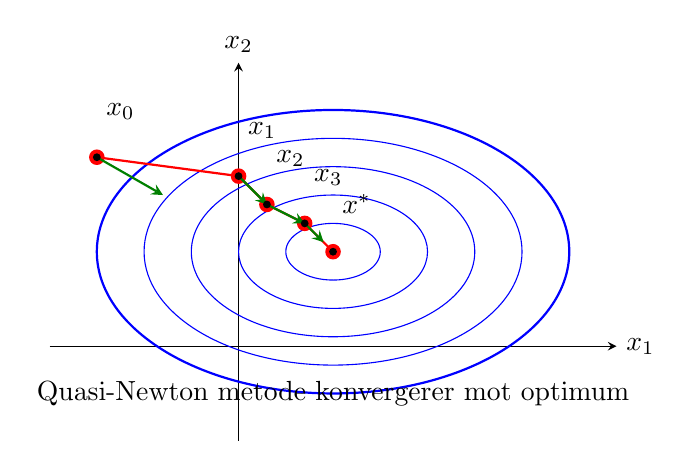
\begin{tikzpicture}[
      scale=1.2,
      >=stealth,
      point/.style={circle,fill=black,inner sep=1pt},
    ]

    % Koordinatsystem
    \draw[->] (-2,0) -- (4,0) node[right]{$x_1$};
    \draw[->] (0,-1) -- (0,3) node[above]{$x_2$};

    % Elliptiske nivålinjer for en kvadratisk funksjon
    \draw[blue, thick] (1,1) ellipse (2.5 and 1.5);
    \draw[blue] (1,1) ellipse (2 and 1.2);
    \draw[blue] (1,1) ellipse (1.5 and 0.9);
    \draw[blue] (1,1) ellipse (1 and 0.6);
    \draw[blue] (1,1) ellipse (0.5 and 0.3);

    % Optimeringsbane
    \draw[mark=*, red, thick, mark size=2pt] plot coordinates {
        (-1.5, 2)
        (0, 1.8)
        (0.3, 1.5)
        (0.7, 1.3)
        (1, 1)
      };

    % Gradient piler
    \draw[->, green!50!black, thick] (-1.5, 2) -- (-0.8, 1.6);
    \draw[->, green!50!black, thick] (0, 1.8) -- (0.3, 1.5);
    \draw[->, green!50!black, thick] (0.3, 1.5) -- (0.7, 1.3);
    \draw[->, green!50!black, thick] (0.7, 1.3) -- (0.9, 1.1);

    % Legg til punkter for tydelighet
    \node[point, label={[shift={(0.3,0.3)}]$\symbf{x}_0$}] at (-1.5, 2) {};
    \node[point, label={[shift={(0.3,0.3)}]$\symbf{x}_1$}] at (0, 1.8) {};
    \node[point, label={[shift={(0.3,0.3)}]$\symbf{x}_2$}] at (0.3, 1.5) {};
    \node[point, label={[shift={(0.3,0.3)}]$\symbf{x}_3$}] at (0.7, 1.3) {};
    \node[point, label={[shift={(0.3,0.3)}]$\symbf{x}^*$}] at (1, 1) {};

    % Figurtittel
    \node at (1, -0.5) {Quasi-Newton metode konvergerer mot optimum};

  \end{tikzpicture}
  \caption{Illustrasjon av Quasi-Newton-iterasjoner som konvergerer mot løsningen langs en ikke-lineær vei. De elliptiske konturene representerer nivålinjer for objektfunksjonen, og punktene viser iterasjonene fra \(\symbf{x}_0\) til den optimale løsningen \(\symbf{x}^*\).}
  \label{fig:quasi_newton_convergence}
\end{figure}

\subsection{Konvergens}
Under passende betingelser viser Quasi-Newton metoder superlineær konvergens:

\[
  \lim_{k \to \infty} \frac{\|\symbf{x}_{k+1} - \symbf{x}^*\|}{\|\symbf{x}_k - \symbf{x}^*\|} = 0
\]

Selv om denne konvergensraten er langsommere enn Newtons kvadratiske konvergens, er kostnaden per iterasjon betydelig lavere, noe som gir en mer effektiv algoritme totalt sett, spesielt for store problemer.

\subsection{Limited Memory BFGS (L-BFGS)}
For høydimensjonale problemer kan lagring av hele Hesse-approksimasjonen være uhåndterlig. Limited Memory BFGS (L-BFGS) lagrer kun de siste \(m\) parene \((\symbf{s}_k, \symbf{y}_k)\) og konstruerer approksimasjonen implisitt.

Dette gir en betydelig hukommelsesbesparelse samtidig som man beholder de gode konvergensegenskapene til BFGS-metoden.

\subsection{Fordeler og begrensninger}
\begin{itemize}
  \item \textbf{Fordeler}:
        \begin{itemize}
          \item Raskere enn gradientbaserte metoder
          \item Lavere kostnad per iterasjon enn Newtons metode
          \item Bygger opp kurvaturinformasjon iterativt
          \item Superlineær konvergens under passende betingelser
        \end{itemize}
  \item \textbf{Begrensninger}:
        \begin{itemize}
          \item Langsommere konvergens enn ren Newton-metode lokalt
          \item Kan kreve flere linjesøk
          \item Sensitiv til nøyaktigheten i linjesøket, spesielt for DFP
        \end{itemize}
\end{itemize}

For å sikre at Hesse-approksimasjonen forblir positiv definit, er det viktig at:

\begin{itemize}
  \item \(\symbf{y}_k^T\symbf{s}_k > 0\) (oppfylt under sterke Wolfe-betingelser)
  \item Initialmatrisen \(\symbf{B}_0\) eller \(\symbf{H}_0\) er positiv definit (ofte satt til \(\symbf{I}\))
\end{itemize}

En vanlig tilnærming for å forbedre ytelsen er å skalere den innledende approksimasjonen:

\[
  \symbf{H}_0 = \frac{\symbf{y}_k^T\symbf{s}_k}{\symbf{y}_k^T\symbf{y}_k}\symbf{I}
\]

Dette gir et bedre estimat for den faktiske skaleringen av den inverse Hesse-matrisen.
